\section{Planning and design process}






The development process involved several stages, including planning, design, implementation, testing and deployment. We started out with an introduction meeting with FiiZK.

\subsection{First meeting}
In the first meeting, we got to know each other. We went over all the necessary details of what the project should include. We discussed and cleared up various uncertainties the group members had about the project. We also got a better understanding of the purpose of the project, as they explained their dissatisfaction with their current methods for configuration file management.


\subsection{Pre-project plan}

The pre-project plan was an essential component of our project management approach, providing a roadmap for the successful execution of the project. It served as a guiding document that outlined the project's objectives, scope, timeline, resources, team roles and key milestones. \\

\noindent
Furthermore, the plan served as a communication tool, facilitating discussions and negotiations with the client, and stakeholders. It ensured that everyone involved in the project had a shared understanding of the project's scope, objectives, and deliverables, and helped us manage expectations effectively.  



\subsection{Design}

Creating wireframes with the feedback of the client before coding was a deliberate decision made to ensure effective communication and alignment with the client's requirements and vision. By creating wireframes, we wanted to visually represent the proposed design and functionality to allow the client to provide feedback and suggestions early in the development process, allowing for any necessary modifications or adjustments to be made before proceeding with the actual coding. 


\subsubsection{Target audience}
An important element in the design decision-making process was the identification of the user group. Specifically, the intended users are individuals who predominantly operate within a computer-based environment and are accustomed to user interfaces that prioritize sleek, futuristic aesthetics and efficient functionality. In light of this, our design sought inspiration from similar interfaces.


\subsubsection{Wireframes}

Wireframes played a critical role in the initial stages of our project, where we worked closely with the client to agree on the design and functionality of the web application. These sketches have also helped us to quickly iterate through different design ideas and gather feedback from the client. This ensured that the client was fully aware of what to expect from the finished product, and it also helped our development team to work more efficiently by having a clear understanding of the requirements from the start. The wireframes can be seen in \autoref{wireframes:signin}.

%I tried to expand this section, it is pretty similar to the current one but i added some more stuff. we could swap the current one for this one, or just remove it and stick to the current one, i just didnt want to swap it myself without hearing your opinions

%Wireframes played a critical role in the initial stages of our project, where we worked closely with the client to agree on the design and functionality of the web application. These sketches were used to quickly iterate through different design ideas and gather feedback from the client, ensuring that they had a clear understanding of what to expect from the finished product. The wireframes also helped our development team to work more efficiently by having a clear understanding of the requirements from the start, as seen in \autoref{wireframes:signin}. In order to ensure a smooth and efficient development process, wireframes were utilized to separate the design phase from the coding phase. By creating wireframes prior to the coding phase, the design process was effectively isolated, enabling us to produce a practical and visually appealing design. During the coding phase, the wireframes were used as a reference template, simplifying the translation of the design into code. This approach allowed for a clear distinction between the creative aspects of design and the more logically-oriented aspects of coding.


\subsection{Client meetings}

We held regular meetings with the client to plan the next sprint and discuss important decisions. These meetings were vital in ensuring effective communication and collaboration between our team and the client. \\

\noindent
During the sprint planning meetings, we reviewed the progress of the previous sprint, identified any challenges or roadblocks, and set clear objectives and goals for the upcoming sprint with the client and the supervisor. This also included clarifying project requirements, design choices, and technical decisions. 

\subsection{Research}

The client granted us the autonomy to determine the most appropriate technologies to utilize for the web application, server, and database. Our initial meetings were focused on this topic. \\

\noindent
The decision on the tech stack was made after careful consideration and evaluation of various factors during the early stages of the project. Our team conducted thorough research and analysis to identify the most suitable technologies for the project's requirements, taking into account factors such as scalability, performance, ease of use, maintainability, industry trends, and compatibility with the project's goals and objectives. We also considered the team's expertise and familiarity with different technologies to ensure smooth development and implementation. 

\subsection{Current state-of-the-art}

During the initial phases of our bachelor’s project, we conducted a comprehensive review of state-of-the-art projects that were similar to our own. The purpose of this review was to gain insights into existing solutions, identify potential gaps or opportunities for improvement, and ensure that our project would be innovative and relevant within the current landscape. \\

\noindent
Despite a thorough search, we were unable to identify any other products that fully met our specific needs. As a result, we decided to explore NoSQL databases for design inspiration, as they offer a structure that closely resembles a JSON file. 

\noindent Although we did not find any existing products that fully met our project's requirements, we did come across a few products that addressed certain aspects of the problem. One such example is a web application designed specifically for JSON schema validation. This tool allows users to input a JSON schema and configuration, which will be validated against the schema to ensure compliance. While the web application mentioned provides an important feature for validating JSON schemas, our project aims to offer a comprehensive tool for managing JSON configurations. In contrast to the existing tool, where JSON configurations have to be created manually or with a separate tool before being validated, our product provides a centralized approach where the entire process of configuration management can be carried out seamlessly with a single tool. This gives our product a significant advantage in terms of efficiency and simplicity, offering a more streamlined and effective solution for JSON configuration management.

\subsubsection{Firebase}

As part of our research, we investigated Firebase for design inspiration. We were interested to see how one of the most popular and widely used NoSQL databases handles traversal through a recursive or hierarchical JSON-like structure. \autoref{firebase:figure}

\begin{figure}[!ht]
   \begin{minipage}{1\textwidth}
     \centering
     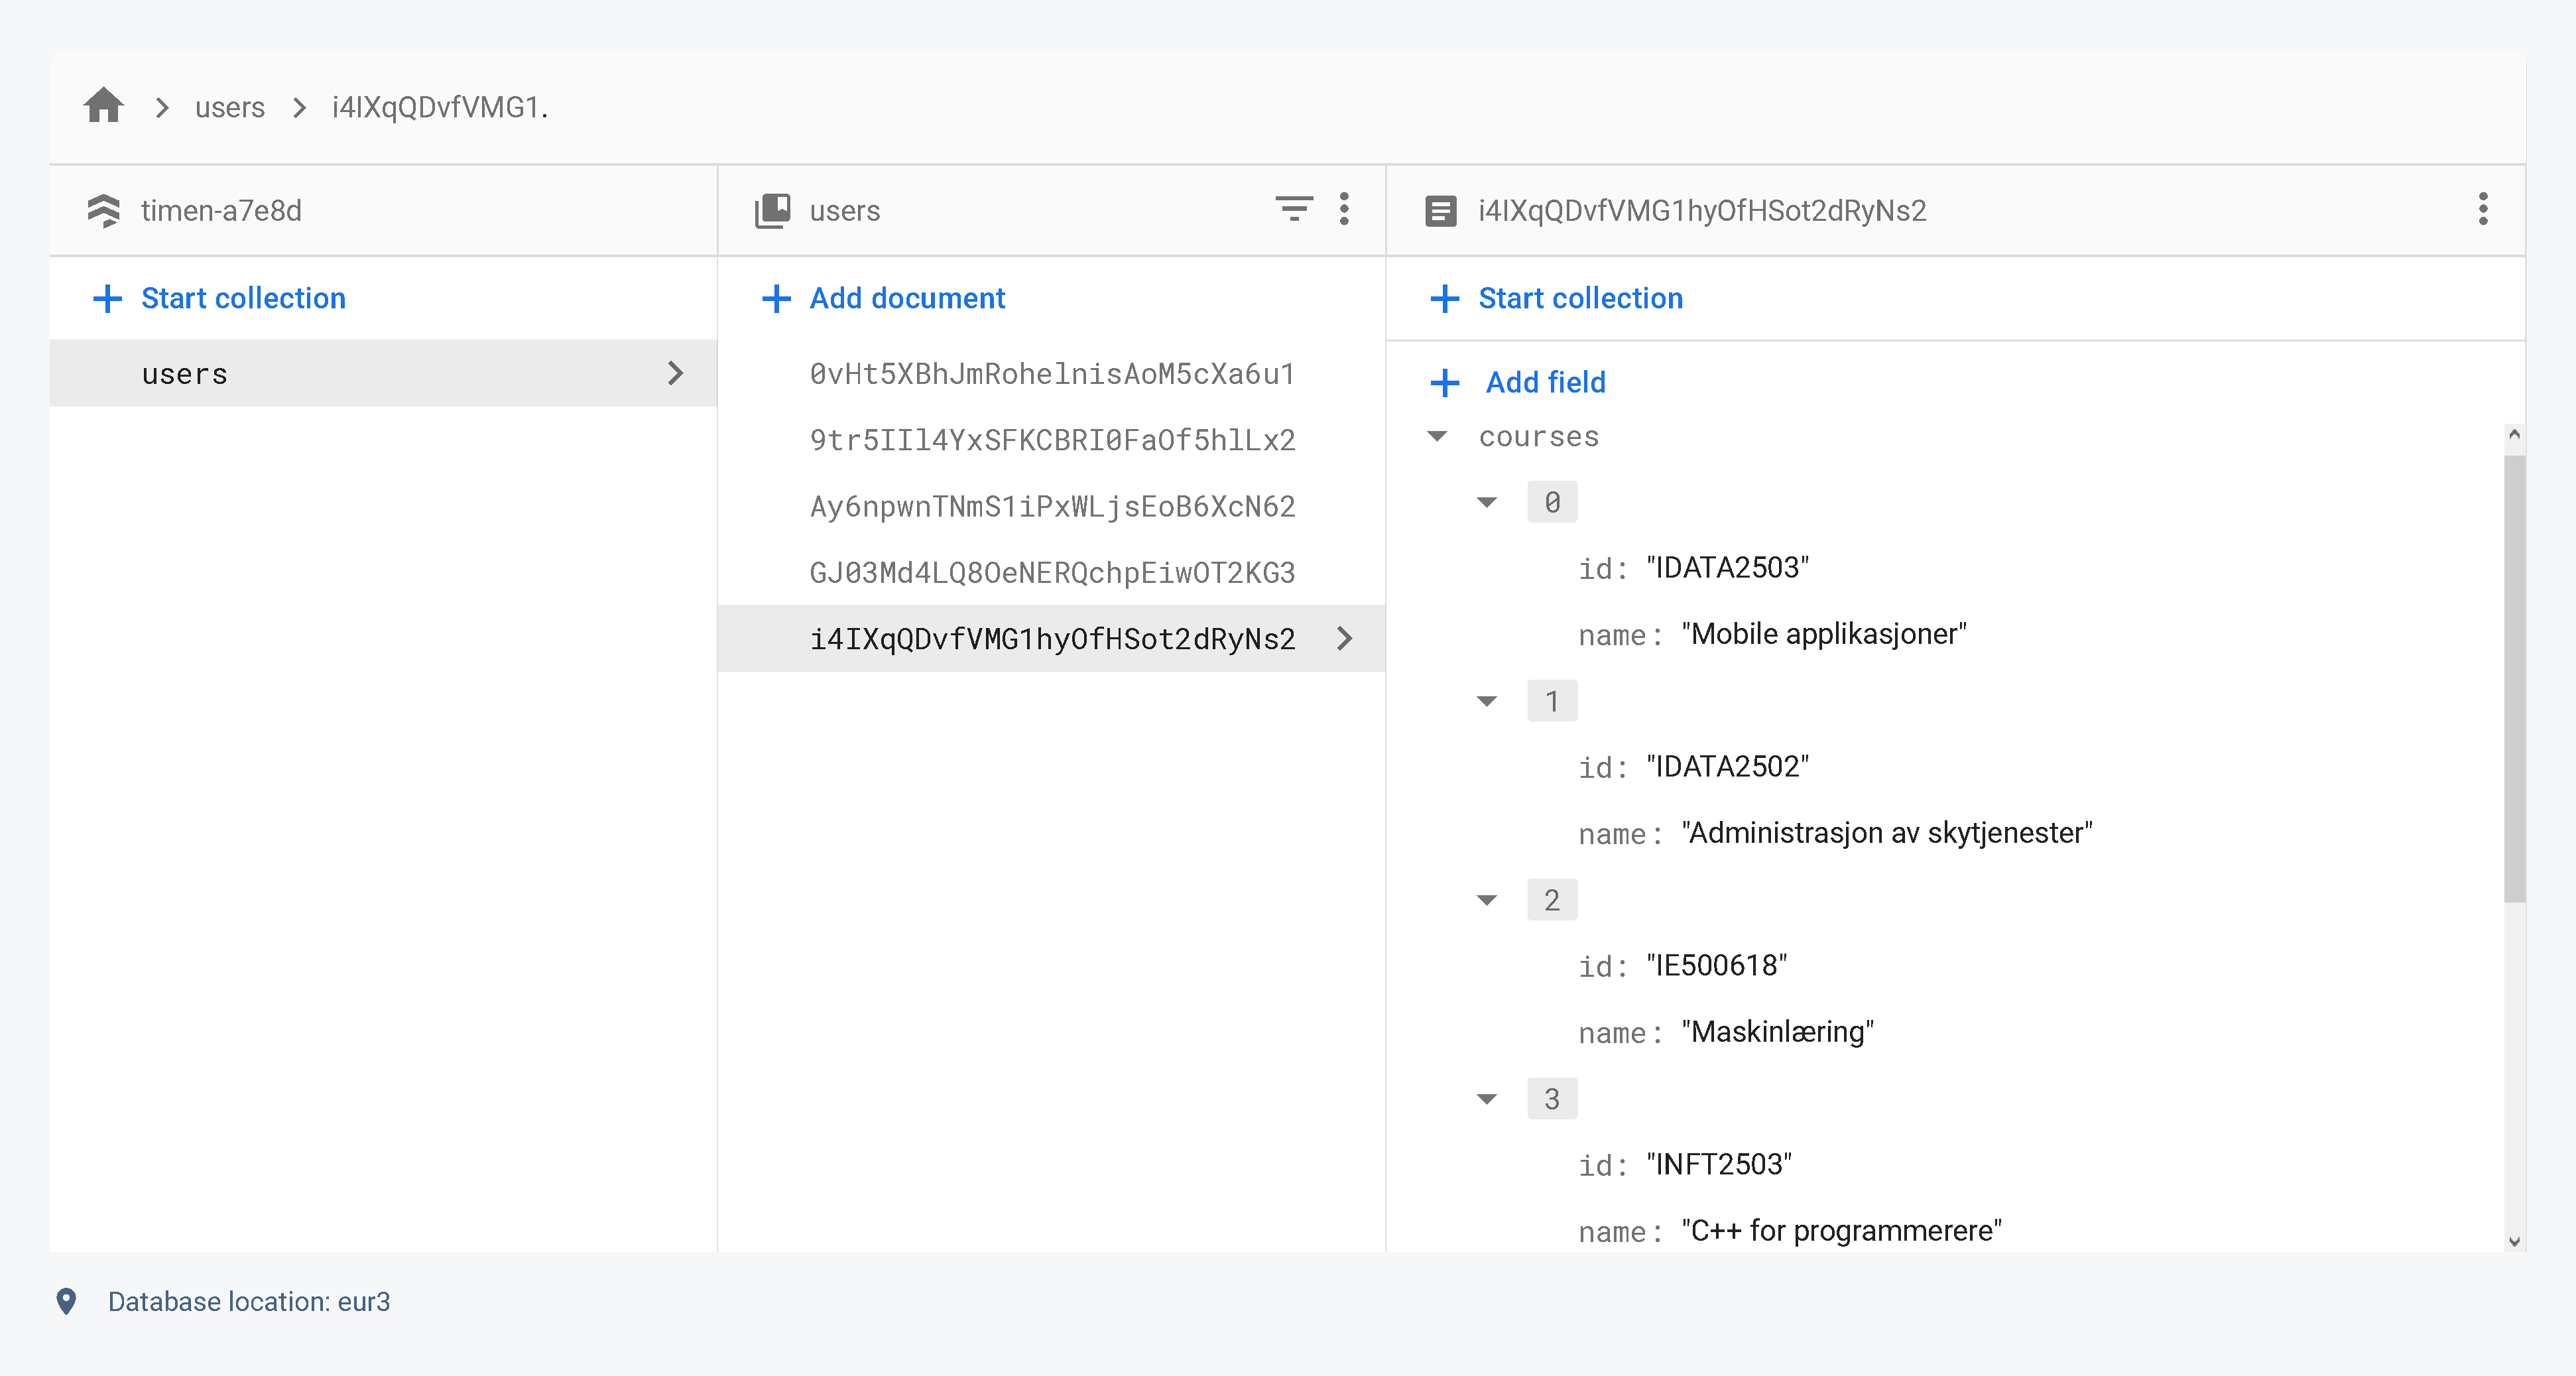
\includegraphics[width=.85\textwidth]{Figures/Firebase-console.pdf}
     \caption{Firebase Cloud Firestore UI}\label{firebase:figure}
   \end{minipage}\hfill
\end{figure}

\noindent 
We conducted a detailed analysis of Firebase’s methods for displaying, traversing, and updating data within a recursive or hierarchical structure. We then adapted and applied these concepts to our own design, drawing inspiration from Firebase's proven methods to efficiently display and manage data with infinite nesting levels. 


%%%%%%%%%%%%%%%%%%%%%%%%%%%%%%%%%%%%%%%%%%%%%

\section{Tools and technology stack}

\subsection{Next.js}

One of the requirements for our web application was that it needed to be performant, scalable, and compatible across multiple devices and platforms. Next.js enabled our team to achieve these goals while streamlining the development process. The project had a strict deadline, and the client wanted the application to be available as quickly as possible. With Next.js, we could leverage its hybrid rendering approach and built-in features to expedite the development process, ensuring that the project would be completed on time. \\

\noindent
Next is a modern web development framework built on top of React developed by Vercel. In Next, user interfaces are constructed using components, which are self-contained, reusable pieces of code which makes it easy to build complex views while maintaining a clean and modular codebase. The development experience with Next.js is further enhanced by features such as hot module replacement and automatic code-splitting. \cite{NextjsDocs}

\subsection{NextAuth}

We’ve chosen NextAuth as our authentication solution. One of the primary factors behind choosing NextAuth was its seamless integration with Next and its ability to  efficiently implement an authentication system without facing compatibility issues or the need for extensive customizations. \\

\noindent
NextAuth offers built-in support for a wide range of popular authentication providers, such as Facebook and Microsoft, in addition to those specifically requested by the client, such as Google, GitHub and a password-less email sign in. \cite{nextauth2022asiuwhu}

\subsection{Chakra UI}

The selection of Chakra UI as the UI library was based on its vast set of customizable components that adhere to modern UI/UX best practices. These components facilitate the creation of a visually appealing and user-friendly interfaces for the application. \cite{chakraui_offical} Additionally, Chakra UI offers seamless integration with Next.js and React frameworks. 

\subsection{tRPC}

The decision to utilize tRPC as the chosen tool for building the API was based on its modern and robust features that allow for the implementation of type-safe APIs across both the front-end and back-end components of the application. \cite{devto_tRPC} With the use of TypeScript with tRPC, the API development process benefits from enhanced typing and code completion capabilities, ensuring a higher degree of code reliability and maintainability. 

% The adoption of tRPC aligns with contemporary best practices in web development, facilitating the construction of a secure and efficient API for the project.

\subsection{TanStack Query}
\label{sec:tanStack_query}

We leveraged TanStack Query, a powerful data fetching and state management library, in combination with tRPC to handle data operations in our web application. tRPC utilizes TanStack Query to provide convenient query hooks for each endpoint, streamlining our server communication. \\

\noindent
With tRPC's integration of TanStack Query, we gained access to query hooks that corresponded to our application's endpoints. These hooks facilitated type-safe and declarative data fetching from the server, ensuring efficient and error-free communication. \cite{devto_tanstack_query} \\

\noindent
Furthermore, TanStack Query's caching mechanisms were seamlessly integrated into the query hooks provided by tRPC. The query hooks automatically managed server response caching and updated the cache when data changes occurred. This optimized caching approach minimized redundant network requests and significantly improved our application's performance.

\subsection{Prisma and the DB solution}

Prisma is an open-source ORM library that simplifies database access and management. It provides an abstraction layer between the application code and the database. It supports popular databases like PostgreSQL, MySQL, SQLite, and more. \\

\noindent
Prisma also has a type-safe query builder that reduces the risk of SQL injection attacks and completely removes the need to write raw SQL queries that could be error-prone and time-consuming. It's schema definition language can sync the current schema with the database schema which greatly streamlines migrations, simplifying the process of evolving and maintaining the database over time. \cite{prisma2022migrate} \\

\noindent
In addition to selecting Prisma as our ORM solution, the team has decided to host the database on a free Render.com PostgreSQL instance. This decision meets our project needs and budget, delivering a quality and secure solution for our client cost-effectively. \cite{render2022pricing}

\subsection{Why store JSON in a relational DB}

Using a relational database to store JSON as a string provides several benefits over using a NoSQL database for this purpose. \cite{Microsoft_JSON_DB_storage} Although NoSQL databases are well-equipped to handle unstructured data such as JSON documents, they lack the rigidity of SQL, which can result in data inconsistencies and compromised data integrity. In contrast, a relational database with SQL provides features such as automatic database delete cascading, constraints, and data types that help ensure data consistency and integrity. Additionally, SQL's rich querying capabilities make it easier to retrieve data in complex ways, which can be particularly useful for complex views or operations. The theory behind this was discussed in \autoref{sec:relational-databases} and \autoref{sec:NoSQL-databases}. 

\subsection{Ajv}

Ajv (Another JSON Schema Validator) is a widely used and popular JavaScript library that provides comprehensive support for JSON schema validation. It is known for its efficiency, performance, and ease of use, and was therefore deemed an appropriate choice for our project. \cite{ajv_general} \\

\noindent
One of the primary factors that influenced our decision to select Ajv was its capacity to accurately validate JSON files against a JSON schema while generating comprehensible and user-friendly error messages. Additionally, it includes a path that enables us to easily navigate to the location of any errors.

\subsection{Vercel}

% * Why we chose to deploy on Vercel \\ 
% * Talk about the advantages of the serverless platform \\ 
% * Tie it to the Theory chapter on serverless and compare to a traditional back-end \\ 
% \todo{Fill in!!!}

We have chosen to deploy our application on Vercel, a cloud platform that offers both static frontends and serverless functions and offers seamless integration with Next.js. \cite{vercel_serverless} With Vercel, we can run and scale our code on-demand without the need to manage our own infrastructure or provision servers, and it automatically scales the application based on demand, which gives high availability and performance without any manual configuration. More theory behind this can be found in \autoref{sec:serverless} on serverless. \\ 

\noindent
Vercel's tight integration with Next.js provides numerous benefits for our deployment process. Firstly, it simplifies the deployment workflow by offering built-in support for Next.js applications, allowing us to deploy our code with ease. Vercel's automatic code-splitting and server-side rendering capabilities optimize the performance and loading speed of our application. Additionally, Vercel leverages edge computing technology, running our code on the Edge, which brings the application closer to the end user, resulting in reduced latency and improved performance. \cite{vercel_edge_network} \\

\noindent
Vercel's CDN (Content Delivery Network) capabilities further enhance the loading speed of static content, ensuring a smooth user experience. By caching and serving static assets from edge locations across the globe, Vercel minimizes the time required to fetch resources, providing faster page load times for users regardless of their geographical location. \\

\noindent
One notable feature that Vercel offers is the ability to preview changes before merging them into the production environment. Each branch in our code repository is assigned a unique preview link by Vercel, allowing us to test and review the branch in a production-like environment without affecting the main application. \cite{vercel_preview_deployments} This preview functionality enables us to validate the changes and ensure they meet our requirements before being merged into the main branch. \\


\subsection{Docker}

Docker is a popular choice for deploying solutions because it provides a consistent and reproducible environment for applications to run in. This makes it easy to deploy, scale and manage applications across different environments. \cite{Docker2022geeksforgeeks} The team’s familiarity with the platform and the client’s requirement to run our solution in their Kubernetes cluster were also important factors in choosing Docker to containerize the app.

\subsection{GitHub, Git-tags and other collaboration tools}

\subsubsection{GitHub}

The team has selected GitHub as the designated code collaboration tool for our project. Leveraging the functionalities offered by GitHub has facilitated seamless collaboration among team members working on the same code-base. The team also has extensive experience with the tool, it's pull requests system and the GitHub Actions ecosystem. 

% This was moved further down
% When a team member intends to merge their branch into the main development branch, they are required to create a pull request. Experienced team members, are granted the authority to approve their own pull requests, however, for less experienced team members, an additional step is implemented wherein another team member is tasked with reviewing the code, and subsequently approving or disapproving the merge request. This process has been instrumental in ensuring that the produced code meets high-quality standards and is adequately documented, contributing to the overall robustness of the project.

\subsubsection{Git Tags}

We have utilized Git tags to capture and document progress. They offer a lightweight and efficient way to mark specific points in the version history of our code repository. By employing git tags, we can effectively track and reference the state of our code-base at the end of each sprint, making it easier to identify and review the changes made during that particular iteration upon the project’s completion. 

\subsubsection{Figma}

In the initial stages of the project, Figma was employed as the design tool. It is a collaborative and cloud-based design tool used to design iterations and get feedback from the client. 

\subsubsection{Jira}

The decision to use Jira as our project management tool was driven mainly by it's comprehensive features set. It is a tools that allows teams to monitor both completed and outstanding tasks, track issues and their progression as well as log working hours. \cite{Ricksoft_Jira} Jira's issue board, a visual representation of the project’s tasks and their status, makes it easier to track progress and prioritize tasks. 

\subsubsection{Confluence}

Confluence was used to create, organize, and share information within the team. It has been primarily utilized to facilitate the sharing of meeting notes, tracking of minimum viable product (MVP) specifications, and documentation of sprint meetings. 

\subsection{Code style}

\subsubsection{Prettier}

We chose to use Prettier as a code formatting tool for our project due to its ability to enforce a consistent code style across the team. Prettier automatically formats code according to predefined rules, ensuring that all team members follow the same code formatting conventions. This helps to eliminate inconsistencies when committing to the repository, improves the overall code readability, and makes it easier for team members to understand and collaborate on each other's code. 

\subsubsection{ESLint}

We’ve decided to utilize ESLint along with the eslint-config-next configuration because it enforces the code style and consistency of the codebase, which makes it easier to read and maintain. The eslint-config-next configuration also includes best practices and rules specific to Next.js development, ensuring that our code adheres to the framework's conventions. \cite{Nextjs_ESLint} 

\subsection{Algorithms and techniques used}

In developing our project, we tried and incorporated advanced algorithms to enhance its functionality and performance. These algorithms play a crucial role in several key areas like improving the overall user experience. 

\subsubsection{Search}

In the project, we investigated the performance of several advanced search algorithms. The idea was to allow the user to miss spell the name of a configuration and still get the desired search result. \\

\noindent
We explored the applicability of advanced string matching algorithms such as Jaro-Winkler and Levenshtein distance in our application. These algorithms are commonly used for comparing and measuring the similarity between strings, which can be useful in various scenarios, including data de-duplication and fuzzy matching. \cite{medium_jaro_levenshtein} However, after thorough testing and evaluation, we determined that these algorithms did not yield satisfactory results for our specific use case. The performance, in terms of result quality, of the search algorithm was found to be no better or even worse than that of a naive algorithm. \\

% For these reasons, the decision was made to abandon this particular enhancement. \\

\noindent
We therefore made the decision to opt for a simpler and more straightforward approach, normal string comparison. By using direct string comparison methods, we were able to achieve the desired level of precision and accuracy in determining string equality. This approach proved to be more effective on the test data we used. \\

\subsubsection{Color generation}

For generating colors programmatically in our application, we developed a custom algorithm inspired by the principles outlined in an article by Martin Ankerl titled "How to create random colors programmatically." The article presents various techniques for generating visually appealing and diverse colors. \cite{color_generation_algo} Our algorithm took inspiration from these techniques to create a color generation process. The algorithm was implemented using the seedrandom JavaScript library, which provided a reliable source of pseudo-randomness. \\

\noindent
The development of the custom color generation algorithm was driven by the client's requirement to ensure visual distinctiveness between the different templates and configurations within our application. The client emphasized the importance of having visually unique and easily distinguishable color schemes for each template and configuration. \\

% \subsection{...Other tools}
% Add any other tools we used under here

\subsection{Communication}

We employed a range of communication tools to facilitate effective collaboration. For internal communication, we utilized Meta's Messenger and Discord, which served as essential channels for planning work sessions, brainstorming ideas, and sharing various files such as concepts and images among team members. \\

\noindent
Externally, we employed email as a formal means of communication with the client and our supervisor. Email was utilized for various purposes, such as scheduling and confirming meetings, sharing meeting agendas, and contacting the external parties for any clarifications or inquiries between the scheduled meetings. 

%%%%%%%%%%%%%%%%%%%%%%%%%%%%%%%%%%%%%%%%%%%%%

\section{Agile development and work allocation}

Following consultation with both the project supervisor and client, the decision was made to utilize the Agile methodology for the project's development. This approach emphasizes an iterative and incremental process, allowing for flexibility and adaptability throughout the project's life-cycle. 

\subsection{Work allocation}

Our project aimed to provide each team member with opportunities to work on various aspects of the project, from front-end to back-end and from design to implementation. It was believed that this approach would promote continuous learning, skill development, and equality among team members. We used Jira to organize the project into different tasks, so the members of the group could assign tasks to themselves and track their progress. 

\subsection{Sprints}

We had set up regular biweekly meetings with the client at the end of each sprint to clarify the goals for the next sprint and to ensure that everyone was aligned with the project's direction. On these meetings we also gathered the client's feedback and set the goals for the next sprint, and made sure that everyone was aware which goals they had to complete until next meeting. \\

\noindent
This approach allowed us to continuously refine and improve the project based on the client's feedback and requirements, while also ensuring that we were meeting their expectations at each stage of development. 

%%%%%%%%%%%%%%%%%%%%%%%%%%%%%%%%%%%%%%%%%%%%%

\section{Development process}

\subsection{User Experience}
As previously mentioned, we conducted research on existing tools that had efficient methods of navigating recursive data. Our goal was to create a professional and polished tool that would provide users with an enhanced user experience. To achieve this, we opted to develop our own browser despite being aware that it would require significant additional time and effort.

\subsection{Quality assurance}

Continuous Integration (CI) played a crucial role in ensuring the quality of our project. We utilized CI to automatically run a build job on every commit, which helped to catch errors and notify the team of any build issues. We ran our CI pipeline on Vercel, a popular tool for CI/CD tool for Next. Additionally, Vercel also offers a preview deployment link from any branch, allowing us to preview our changes before merging them into the main branch. \\

\noindent
We also utilized ESLint, a popular TypeScript linter tool, to catch potential bugs or errors before they can cause issues. To ensure that our code meets the highest possible quality standards, we customized our linting preferences to be particularly stringent. 

\subsection{Code review}

Our team used a code review process to review each other's code and catch any potential issues or misunderstandings before merging into the main branch. 

\noindent
Experienced team members, are granted the authority to approve their own pull requests, however, for less experienced team members, an additional step is implemented wherein another team member is tasked with reviewing the code, and subsequently approving or disapproving the merge request. This process has been instrumental in ensuring that the produced code meets high-quality standards, contributing to the overall robustness of the project.

% \subsection{Pair programming}
% As mentioned, the group had a notable experience gap, with some members having extensive knowledge and familiarity with the technologies and languages used in the project, while others had little to no experience. To address this issue, the team adopted a modified form of pair programming. The more experienced team members took on the role of the "driver," responsible for writing the code while simultaneously explaining the process to a less experienced team member, who acted as the "co-pilot." The co-pilot's task was to challenge the driver's understanding of the process by asking critical questions, which forced the driver to think more deeply and explain their actions more thoroughly.

% \noindent This approach enabled both the driver and co-pilot to learn from each other simultaneously. The co-pilot was able to gain a better understanding of the coding process, while the driver honed their own understanding by articulating it to the co-pilot. The team hoped that over time, the co-pilot would become more involved in the development process as they gained more experience and knowledge. The modified pair programming technique was intended to be an effective means of bridging the knowledge gap and promoting a collaborative learning environment.

